\section{Vorgehen}

Die Vorgehensweise orientiert sich an Scrum, wird jedoch angepasst auf dieses Projekt.
Scrum ist eine agile, inkrementelle Projektmethode, die oft in Softwareentwicklung verwendet wird. Dabei wird in Zeitboxen, die Sprint genannt werden, gearbeitet. Pro Sprint gibt es mehrere Tasks, die bearbeitet werden sollen, sowie Sprintziele. Dies wird in diesem Projekt so gemacht.\cite{wikipedia-scrum}

Normalerweise gibt es tägliche Synchronisationsmeetings. Hier werden diese wöchentlich durchgeführt, ansonsten wird eher asynchron gearbeitet.

Sprintreviews werden durchgeführt im Rahmen der Besprechung der Testatabgaben mit dem Coach. Retrospektiven werden nicht strukturiert durchgeführt, jedoch wird zu Ende jedes Sprints besprochen, ob die Arbeitsweise angepasst werden soll für den nächsten Sprint.

Als Scrum Board wird Microsoft Teams verwendet. Der Backlog wird zu Beginn der Projektes definiert und in einzelne Sprintbacklogs aufgeteilt.

\subsection{Projektorganisation}

Da es sich um eine interdisziplinarische Produktentwicklung handelt, wurde das Team aus jeweils zwei Studierenden aus den Studiengängen \acrfull{elektrotechnik}, \acrfull{informatik} und \acrfull{maschinentechnik} zusammengeführt. In Abbildung \ref{fig:Organigramm} ist die Projektorganisation ersichtlich. 

Im Team wurde Alina Meyer als Projektleiterin gewählt. Zudem benötigt es für die mechanischen und elektrischen Werkstätten in der Hochschule Luzern jeweils einen zuständige Person im Team. Diese wurden Ivan Zimmerman (\acrshort{elektrotechnik}) und Elias von Atzigen (\acrshort{maschinentechnik}) zugeteilt.

Die klare Aufteilung der Rollen ermöglicht es dem Team effizient und zielgerichtet an der Entwicklung des Projekts zu arbeiten. Durch diese Struktur wird gewährleistet, dass jede technische Disziplin angemessen abgedeckt ist und die Kommunikation innerhalb des Teams reibungslos funktioniert.

\begin{figure}[H]
\centering
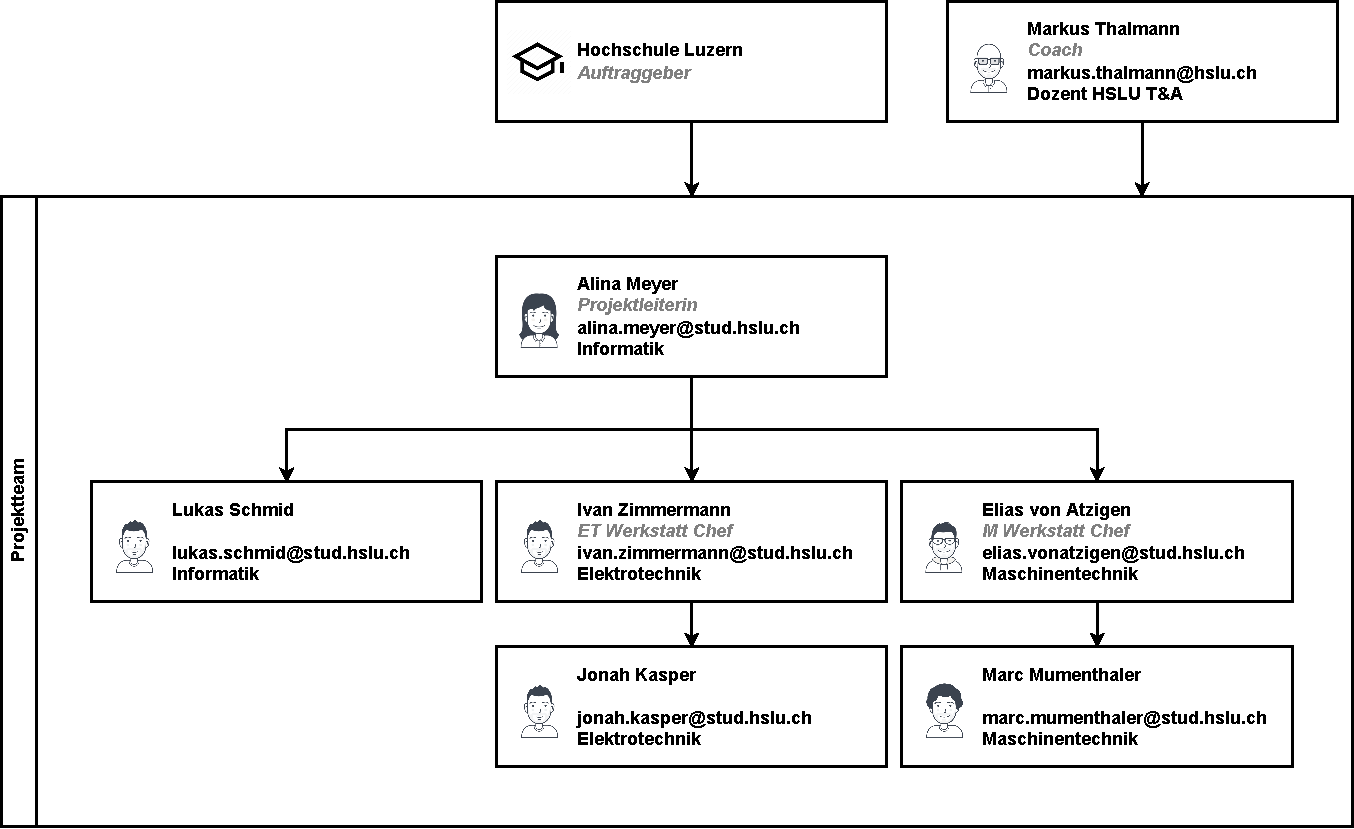
\includegraphics[width=\textwidth]{img/Projektorganisation.pdf}
\caption{Organigramm}
\label{fig:Organigramm}
\end{figure}

\subsection{Datenaustausch}

Zur Zusammenarbeit in diesem Projekt wurde ein Team auf Microsoft Teams erstellt.
Darin ist eine Datenablage, ein Taskboard und ein Chat enthalten. Der Chat wird jedoch weniger verwendet, da die Kommunikation hauptsächlich über WhatsApp erfolgt, damit die Antwortzeiten möglichst kurz sind.

Die Dokumentation wird auf einer eigenen Overleaf Instanz in LaTeX erstellt.

Der erstellte Code wird auf GitHub gespeichert.

Eine detaillierte Auflistung des Datenaustausches und aller Kommunikationsschnittstellen befindet sich im Anhang.
